\documentclass[aspectratio=169]{beamer}

\usetheme[titleformat=allcaps,sectionpage=simple,progressbar=frametitle,background=dark]{metropolis}
\RequirePackage{etoolbox}
\RequirePackage{ifxetex}
\RequirePackage{ifluatex}
\RequirePackage{pgfopts}

\usepackage{color}
\definecolor{background}{HTML}{ffffff}
\definecolor{text}{HTML}{333333}
\definecolor{background}{HTML}{333333}
\definecolor{text}{HTML}{ffffff}
\definecolor{warning}{HTML}{f0ad4e}
\definecolor{success}{HTML}{5cb85c}

\setbeamercolor{progress bar}{fg=success,bg=background}
\setbeamercolor{progress bar in section page}{fg=success,bg=background}
\setbeamercolor{title separator}{fg=warning,bg=text}
\setbeamercolor{normal text}{fg=text,bg=background}
\setbeamercolor{frametitle}{fg=text,bg=warning}
\setbeamercolor{section title}{fg=text,bg=warning}
\setbeamercolor{palette primary}{bg=warning}

\setbeamercolor{titlelike}{fg=text}
\setbeamercolor{author}{fg=text}
\setbeamercolor{date}{fg=text}
\setbeamercolor{institute}{fg=text}

%\usepackage{default}
\usepackage{graphicx}
\usepackage{amssymb}
\usepackage[ngerman,english]{babel}
\usepackage{appendixnumberbeamer}
\usepackage{textcmds}
\usepackage{float}
\usepackage{csquotes}

\usepackage{pgfpages}
%\setbeameroption{show notes on second screen}

% Define block styles
\tikzstyle{decision} = [diamond, color=background, fill=red!20, text width=5em, text badly centered]
\tikzstyle{block} = [rectangle, color=background, fill=blue!20, text width=7em, text centered, rounded corners, minimum height=4em, text centered]
\tikzstyle{cloud} = [ellipse, color=background, fill=green!20, minimum height=2em, text centered, text width=4em]

\title{Interpolation - On the example of the intra-urban Heat island effect in Berlin}
\subtitle{FOSSGIS Seminar}
\date{Janurary 27, 2021}
\author{Anja Doppelmayr \& Malte Heinzelmann}
\institute{Ruprecht-Karls-Universit\"at Heidelberg}

\makeatletter
\def\beamer@framenotesbegin{% at beginning of slide
	\usebeamercolor[fg]{normal text}
	\gdef\beamer@noteitems{}%
	\gdef\beamer@notes{}%
}

\setlength{\metropolis@titleseparator@linewidth}{2pt}
\setlength{\metropolis@progressonsectionpage@linewidth}{2pt}
\setlength{\metropolis@progressinheadfoot@linewidth}{2pt}

\newlength\beamerleftmargin
\setlength\beamerleftmargin{\Gm@lmargin}
\makeatother

\usepackage[export]{adjustbox} 

\usepackage{tikz}
\usetikzlibrary{arrows,positioning,shapes,arrows.meta}

\usepackage[absolute,overlay]{textpos}
\setlength{\TPHorizModule}{\paperwidth} % horizontal unit
\setlength{\TPVertModule}{\paperheight} % vertical unit

\usepackage[
backend=biber,
style=alphabetic,
]{biblatex}
\usepackage{tabularx}
\usepackage{pifont}% http://ctan.org/pkg/pifont

\newcommand{\cmark}{\ding{51}}%
\newcommand{\xmark}{\ding{55}}%

\addbibresource{../writeup/biblatex.bib} %Imports bibliography file

\newenvironment*{env}{}{}

\begin{document}
	\begin{frame}[plain]
		\makebox[0pt][l]{%
			\hspace*{-11mm}
			%\hspace*{-\beamerleftmargin}
			\raisebox{-\totalheight}[0pt][0pt]{%
				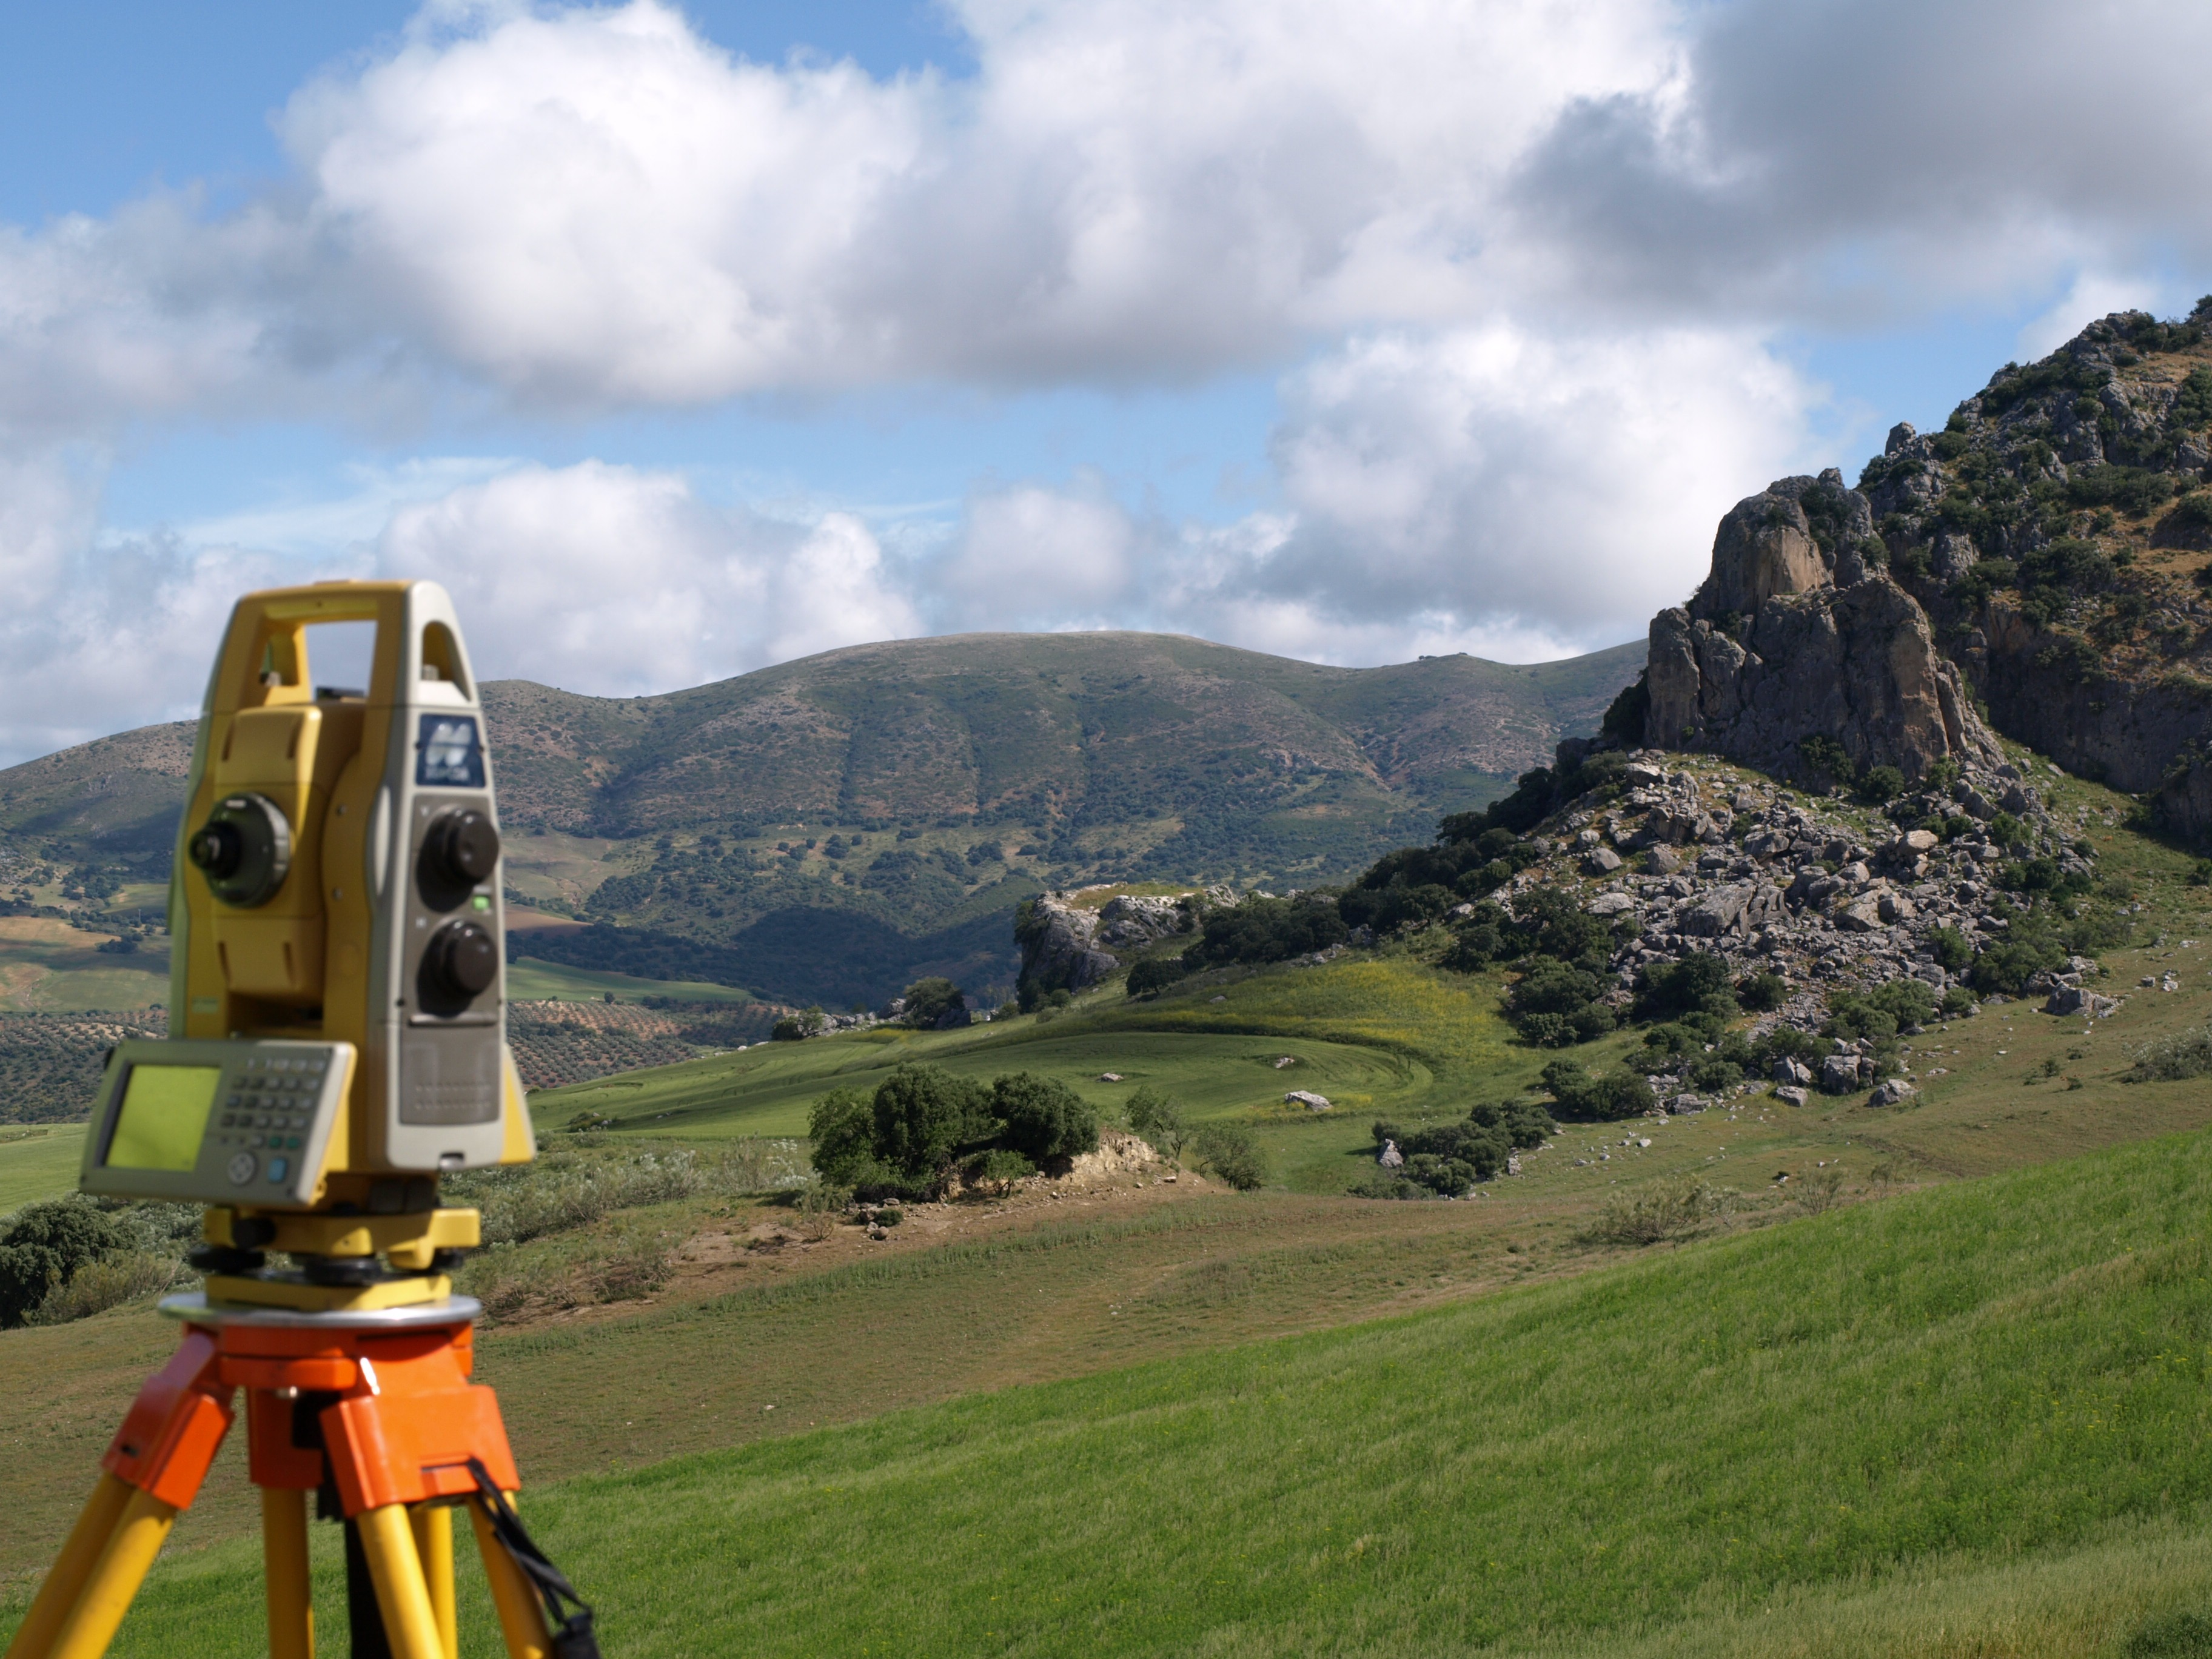
\includegraphics[width=\paperwidth,keepaspectratio]{images/background}
			}
			\hspace*{-\paperwidth}
			\hspace*{-5mm}
			\raisebox{-\totalheight}[0pt][0pt]{%
				
\includegraphics[width=\paperwidth,height=\paperheight]{images/backdrop.png}
			}
		}
		\begin{textblock}{1}[1,1](0.995,0.99)
			\setlength\topsep{0pt}
			\begin{flushright}
				\tiny\color{text} Source: Pixabay (davidph, topography-station-measurement-202278)%
			\end{flushright}
		\end{textblock}
		\titlepage
	\end{frame}

	\begin{frame}{Agenda}
		\tableofcontents[]
	\end{frame}

	% !TeX root = ../presentation.tex

\section{Introduction}
\begin{frame}{What is interpolation?}
	\begin{columns}[T] % align columns
		\begin{column}{.48\textwidth}
			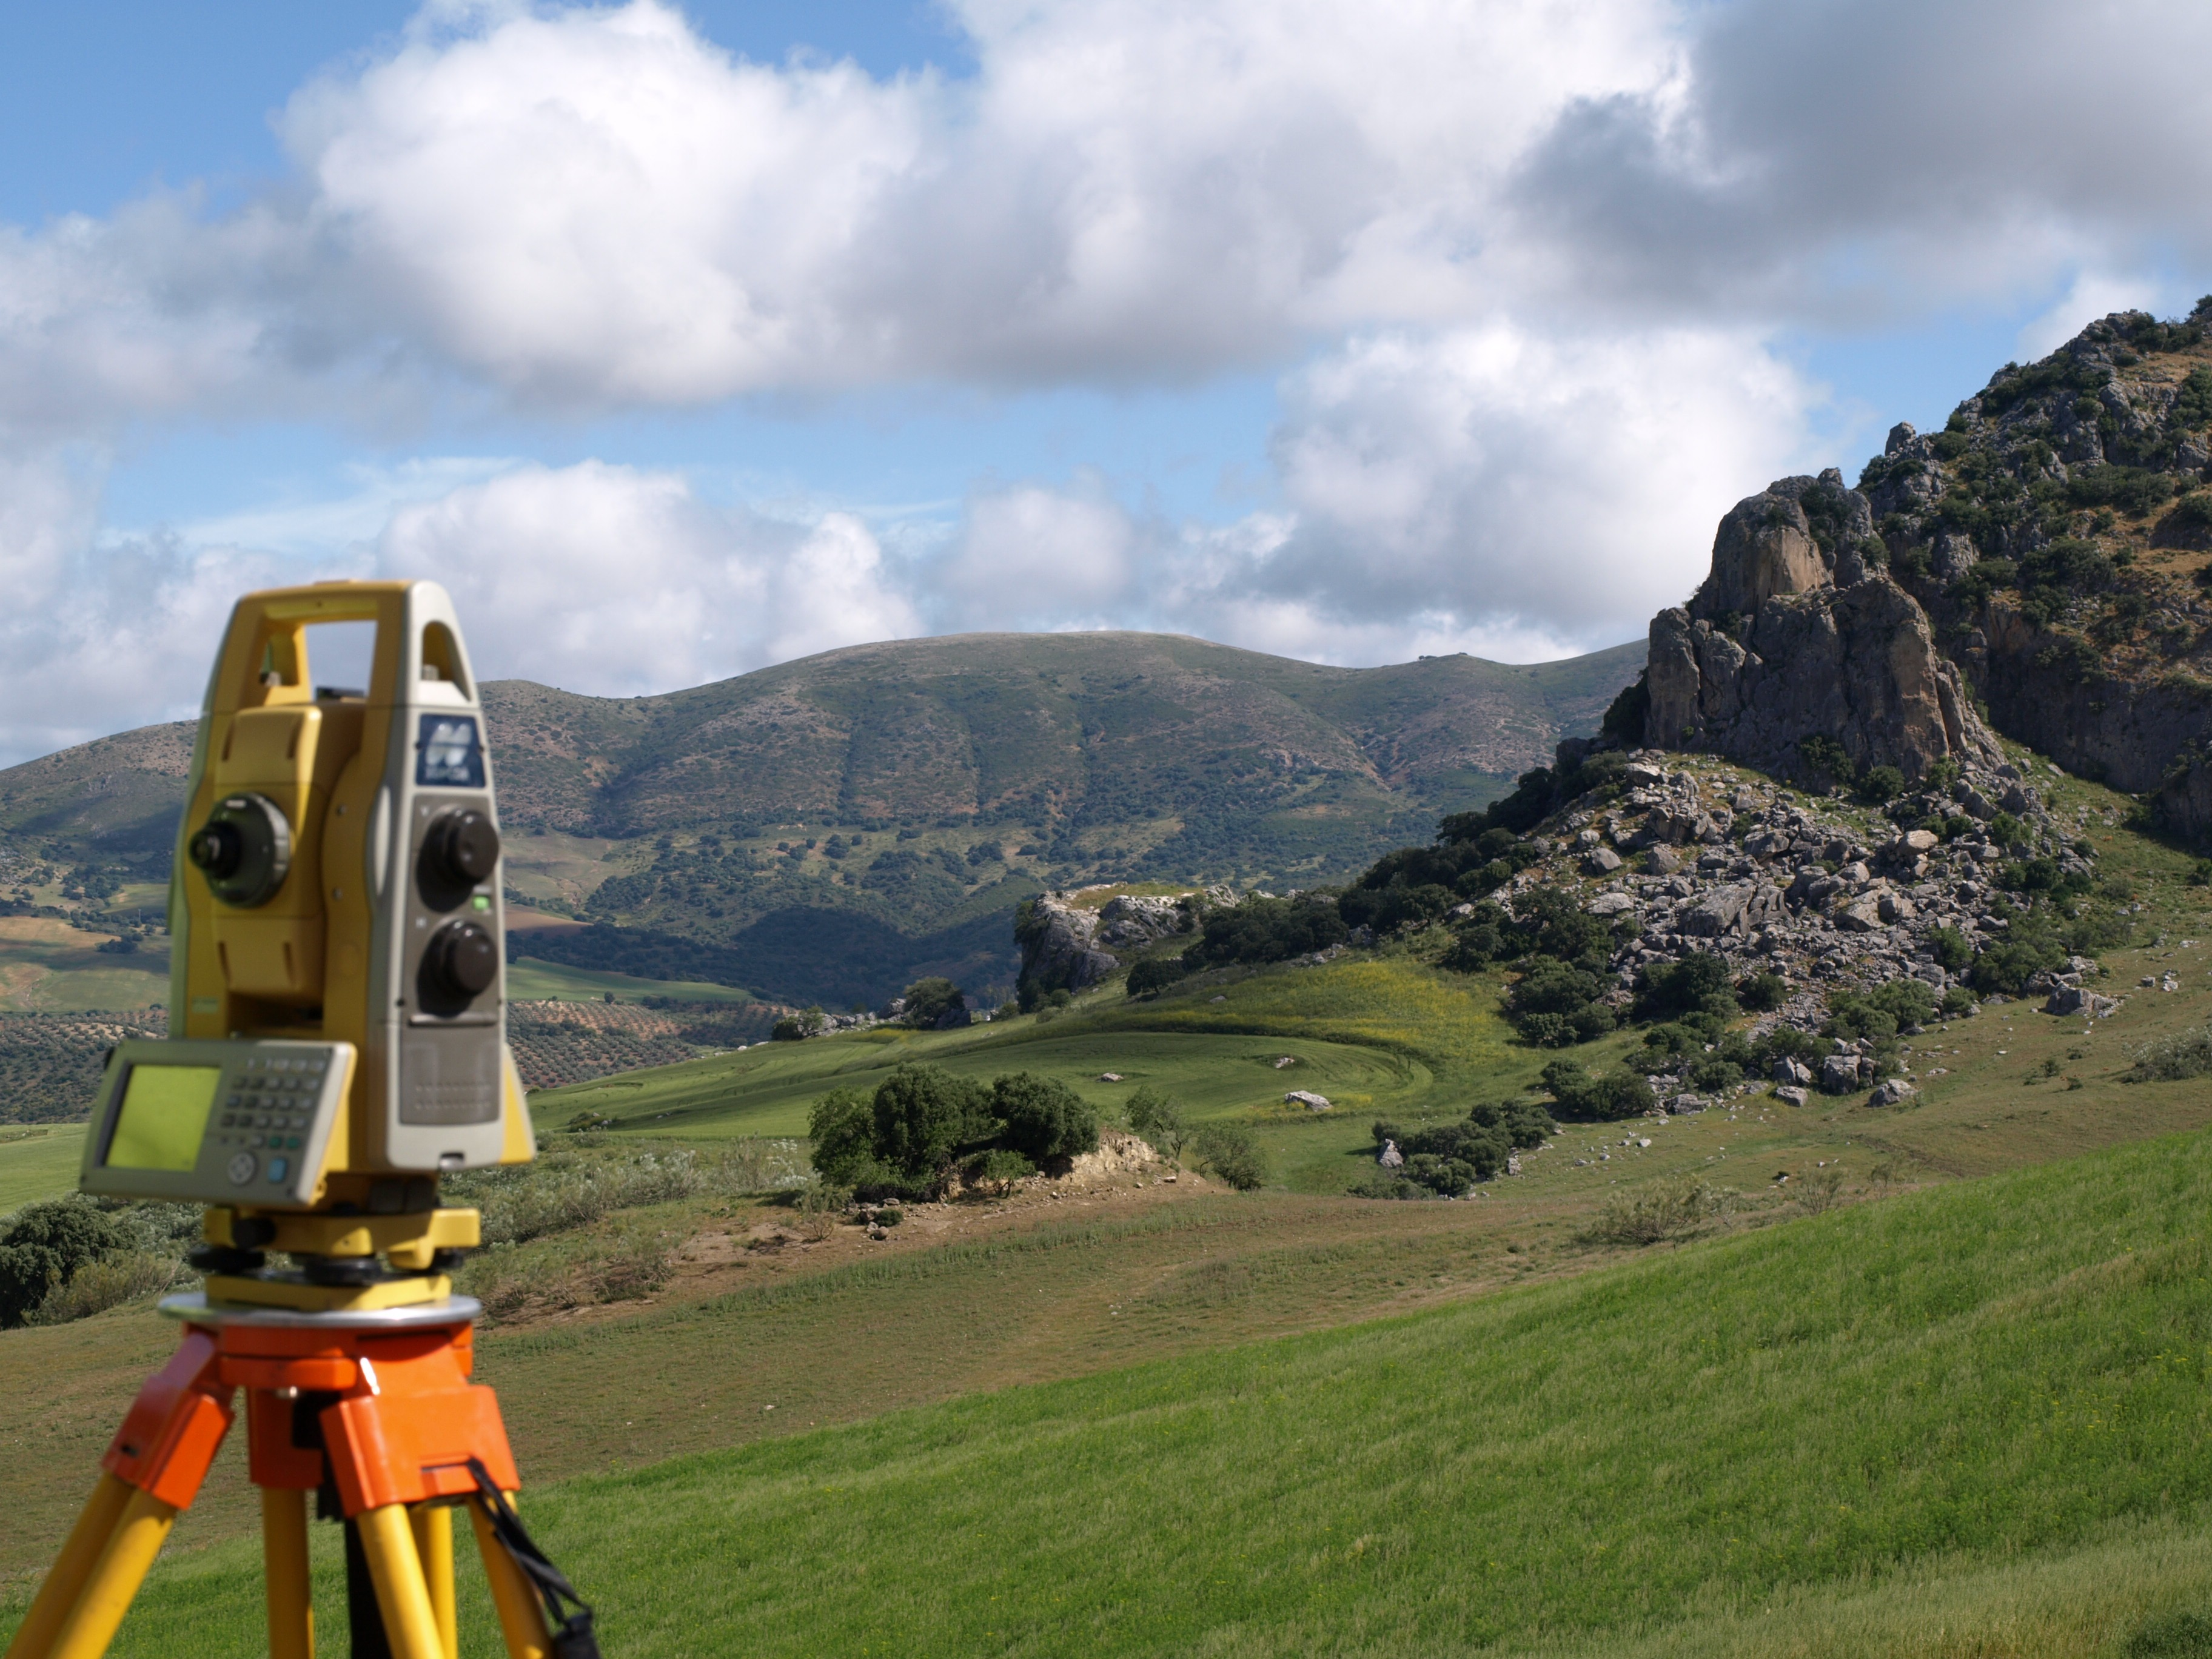
\includegraphics[width=\linewidth]{images/background}
		\end{column}%
		\hfill%
		\begin{column}{.56\textwidth}
			\begin{itemize}
				\item TODO
				\item TODO 2
			\end{itemize}
		\end{column}%
	\end{columns}
	\note{say "hello" now}
\end{frame}
\begin{frame}{This is interpolation!}
\begin{columns}[T] % align columns
	\begin{column}{.56\textwidth}
		\begin{itemize}
			\item TODO
		\end{itemize}
	\end{column}%
	\hfill%
	\begin{column}{.48\textwidth}
		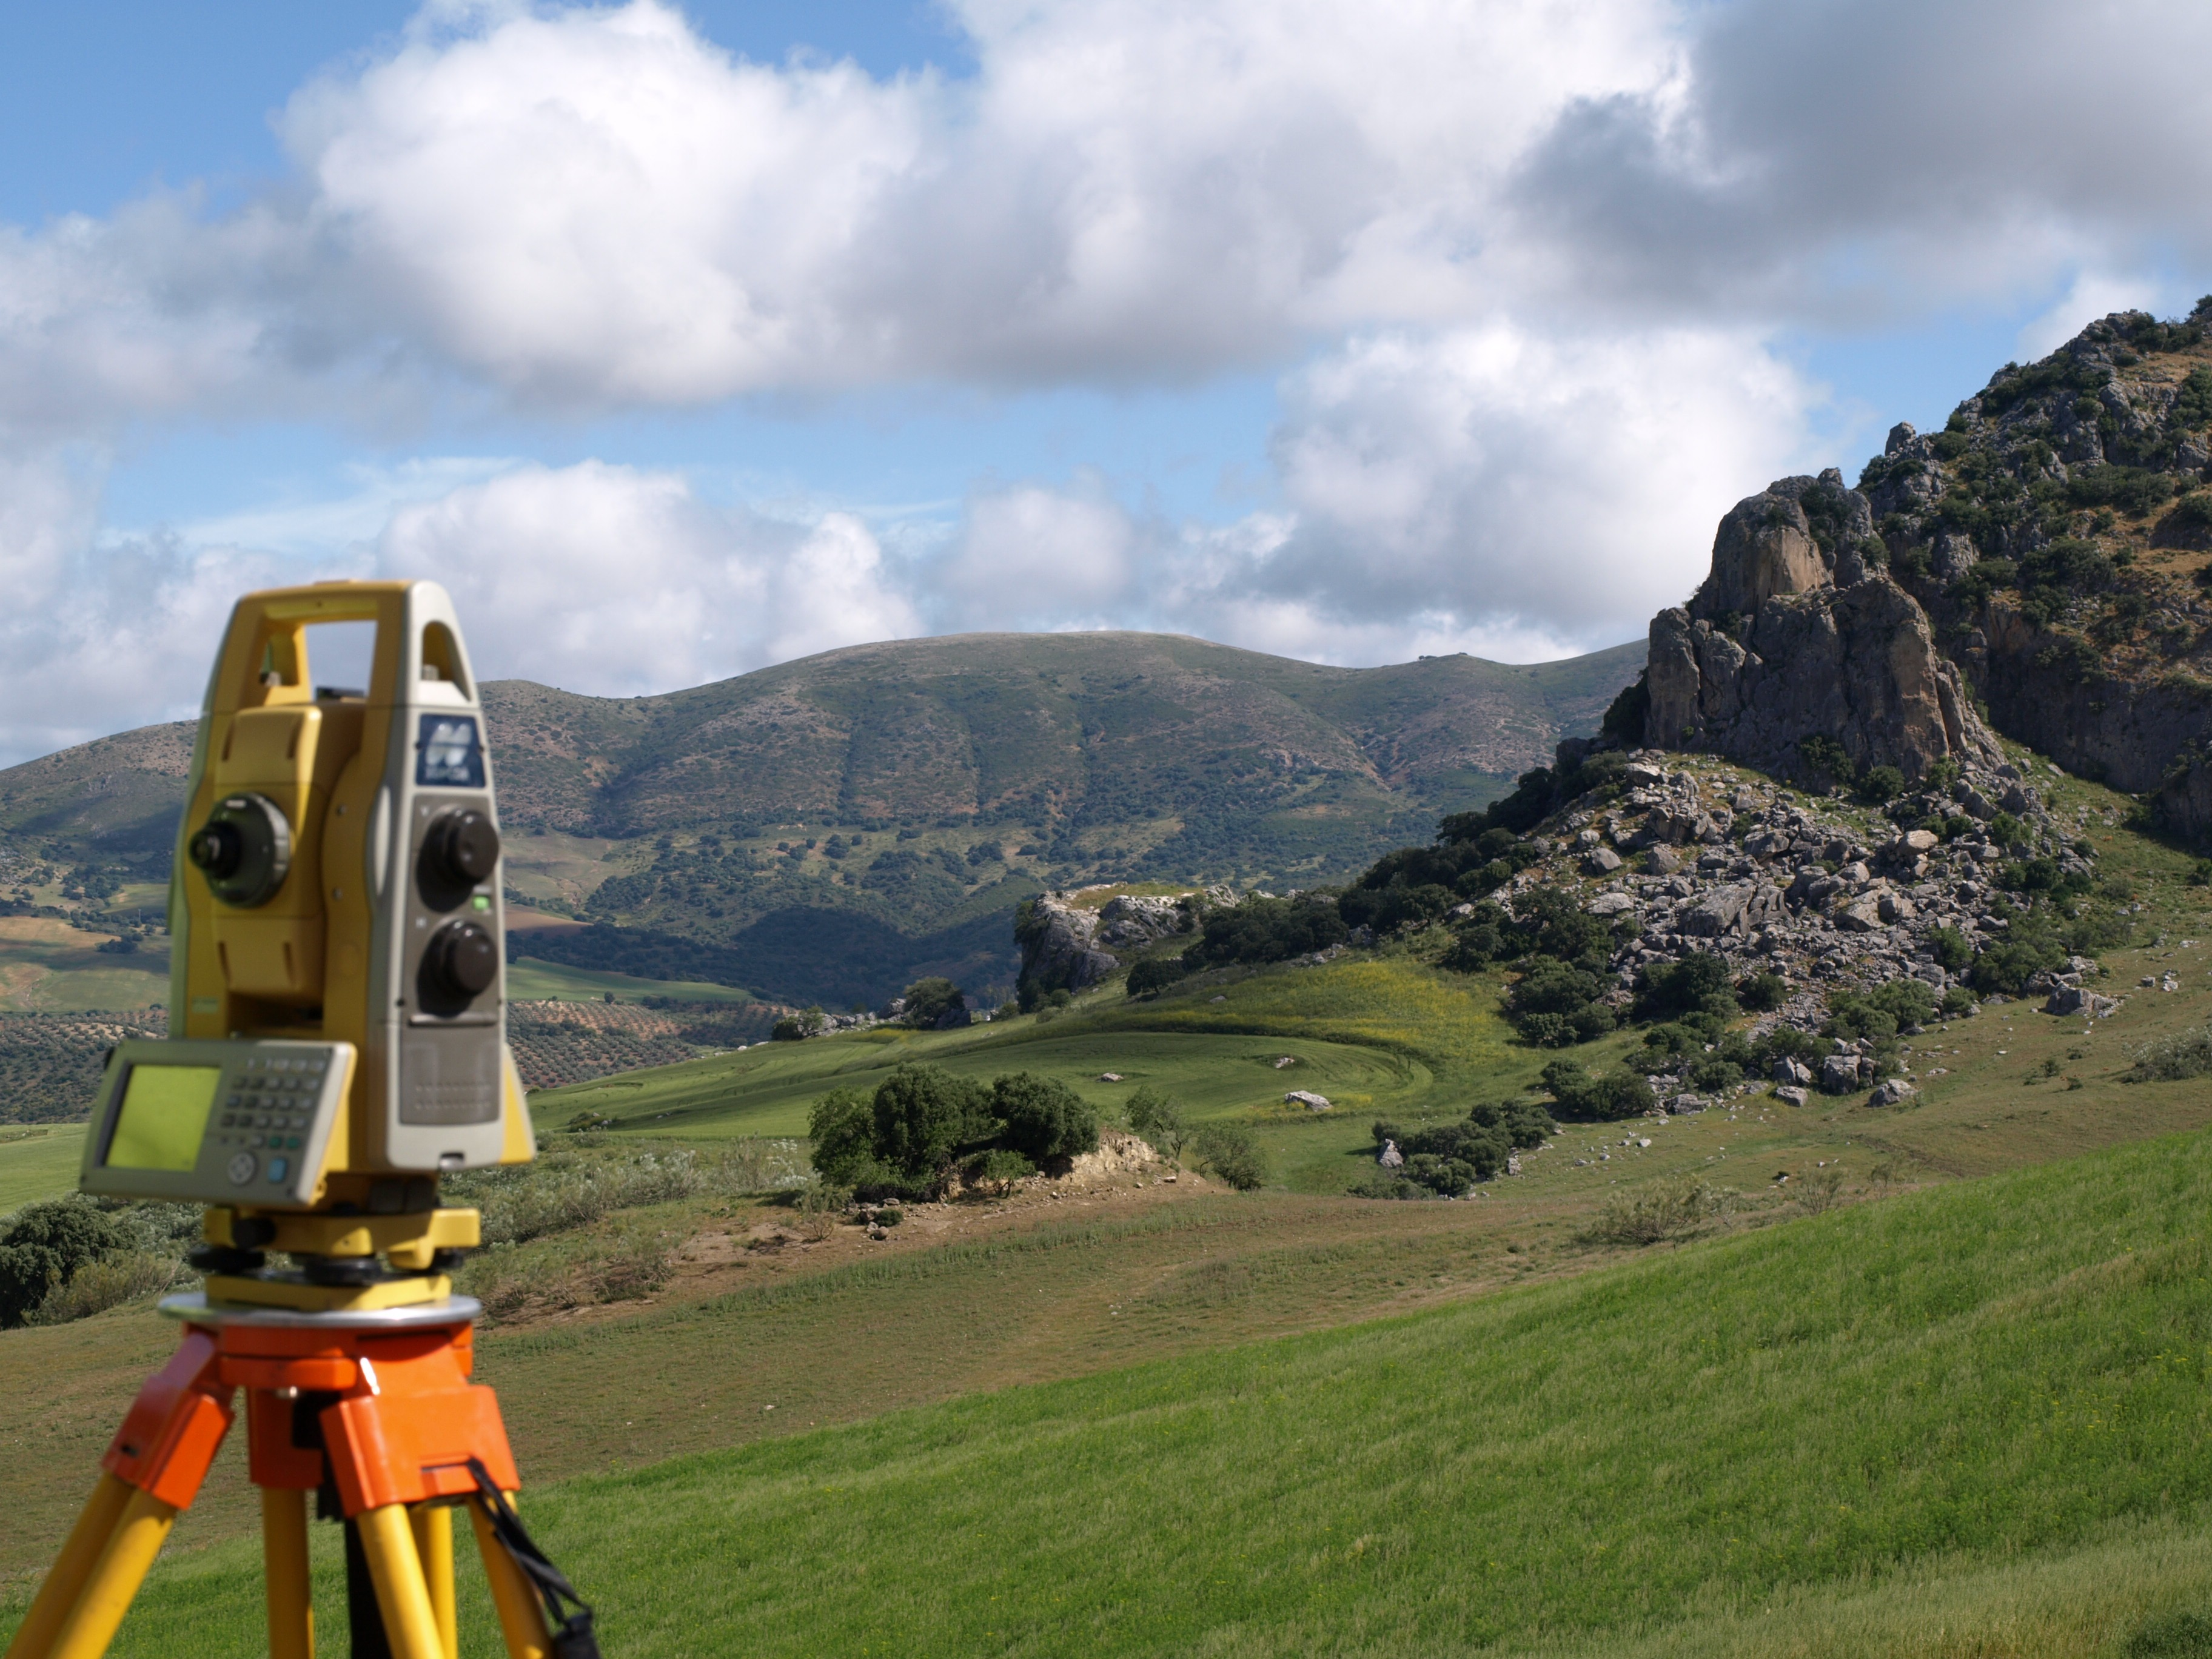
\includegraphics[width=\linewidth]{images/background}
	\end{column}%
\end{columns}
\note{say "hello" now}
\end{frame}

	% !TeX root = ../presentation.tex

\section{Interpolation}
\begin{frame}{Interpolation methods overview}
	\begin{columns}[c] % align columns
		\begin{column}{.5\textwidth}
			\centering
			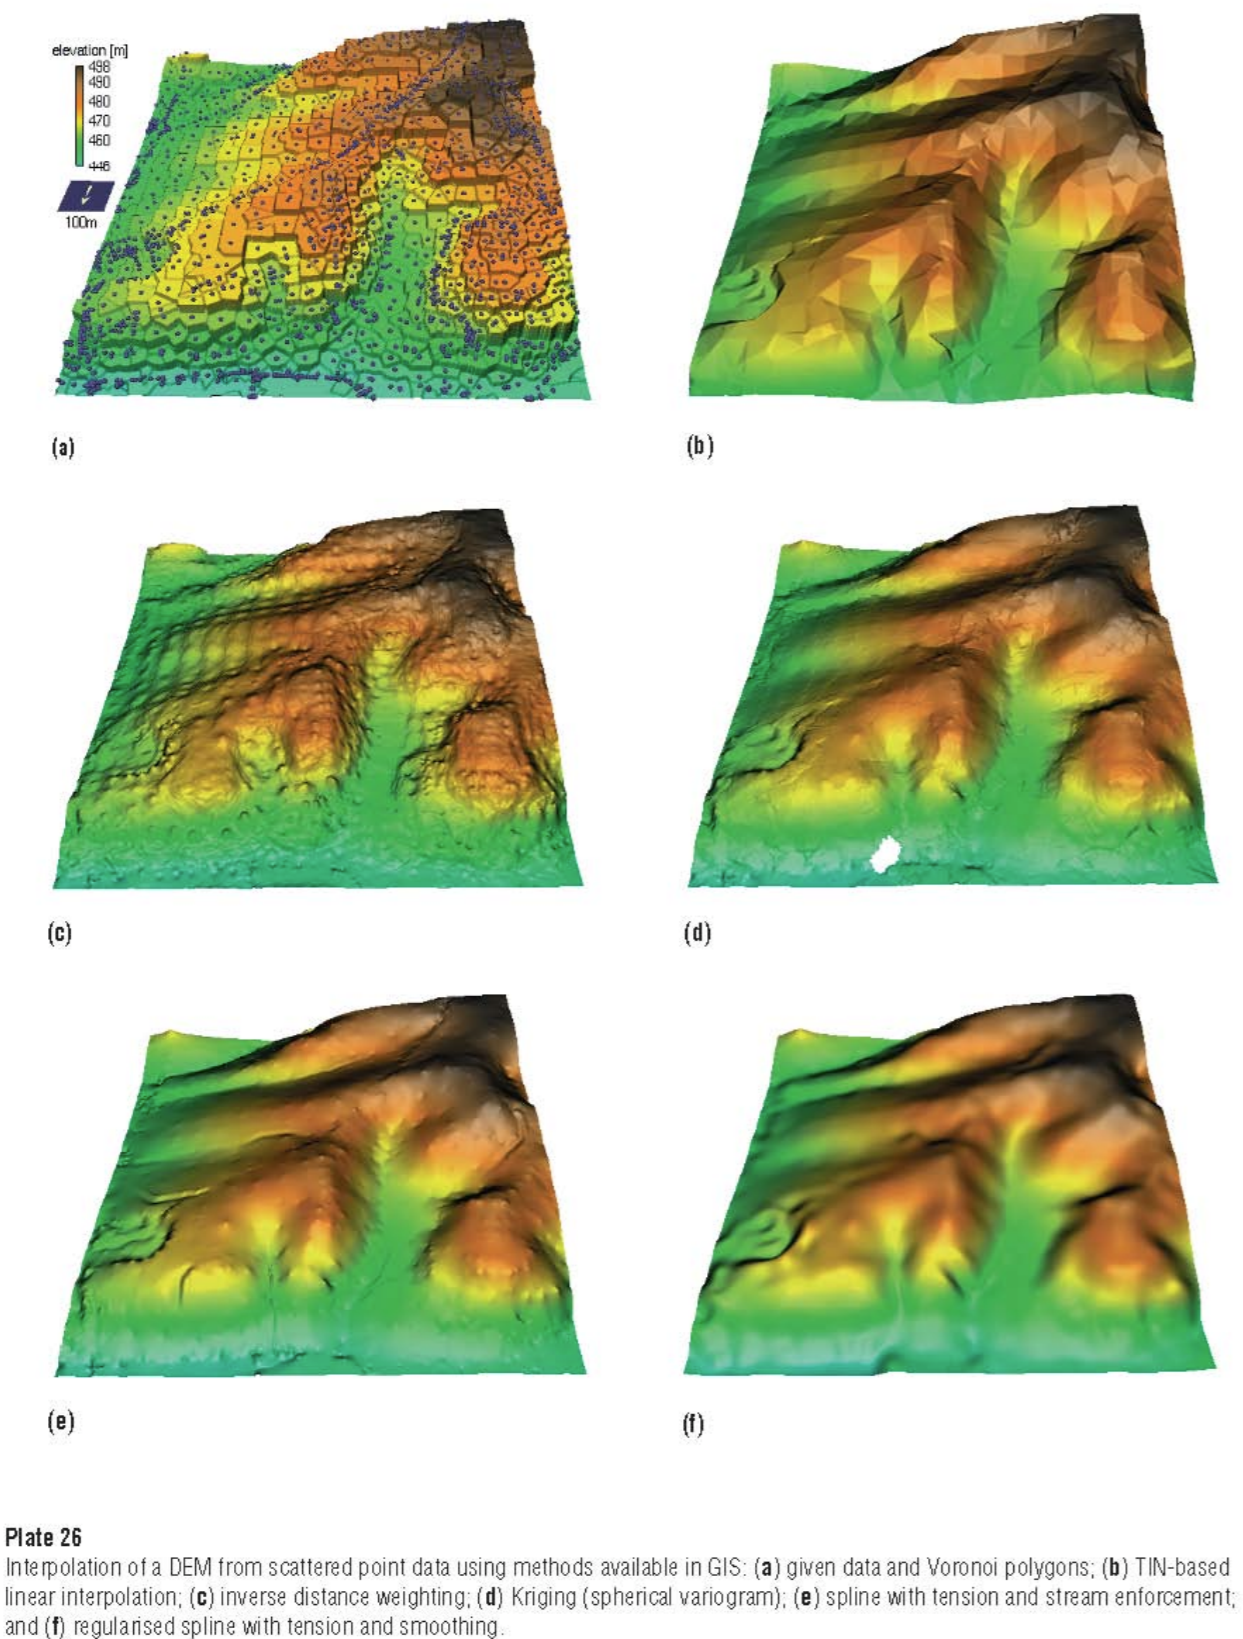
\includegraphics[trim=0 100 0 0,clip,height=.75\textheight]{../writeup/images/dem.png}\\
			\textit{\footnotesize Interpolation with different methods \cite{mitas_spatial_1999}}
		\end{column}%
		\hfill%
		\begin{column}{.5\textwidth}
			\begin{itemize}
				\item Nearest Neigbor (deterministic) <a>
				\item Linear/TIN (deterministic) <b>
				\item IDW (deterministic) <c>
				\item Spline (deterministic) <e \& f>
				\item Kriging (statistical) <d>
			\end{itemize}
		\end{column}%
	\end{columns}\end{frame}
\begin{frame}{Nearest Neighbor}
	\begin{columns}[c] % align columns
		\begin{column}{.52\textwidth}
			\begin{itemize}
				\item Voronoi diagrams
				\item Value is exactly the value of its nearest neighbor
				\item Sharp edges
				\item Inaccurate if known points have a great distance
			\end{itemize}
		\end{column}%
		\hfill%
		\begin{column}{.48\textwidth}
			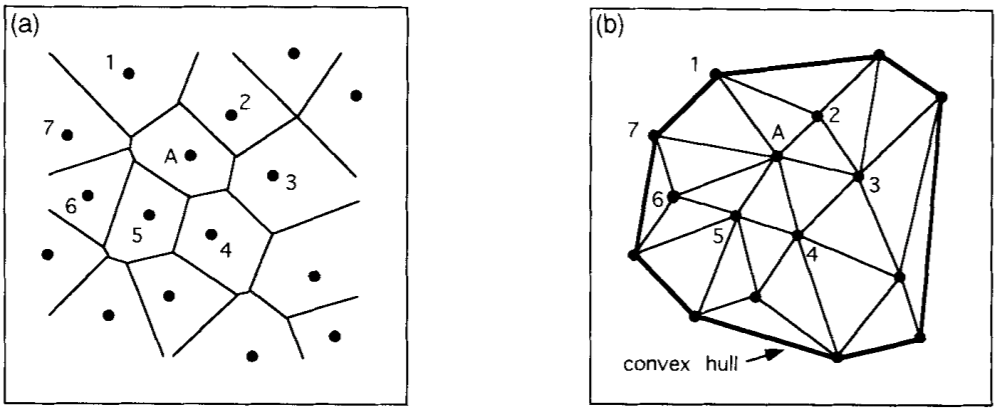
\includegraphics[trim=0 0 294 0,clip,width=\linewidth]{../writeup/images/voronoi_delauny.png}\\
			\textit{\footnotesize Voronoi diagram \cite{sambridge_geophysical_1995}}
		\end{column}%
	\end{columns}
	\note{The basis for this method are so-called Voronoi diagrams. Thereby, „plans“ or polygons, which are produced according to the known point value they refer to. The values within these “planes” are then „filled“ with the same value of the corresponding nearest neighbor (aka. known point).}
\end{frame}
\begin{frame}{Linear/TIN}
\begin{columns}[c] % align columns
	\begin{column}{.48\textwidth}
		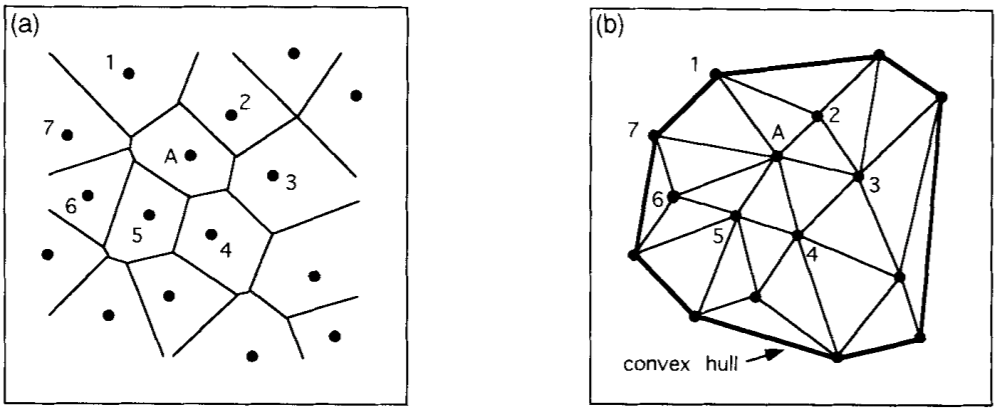
\includegraphics[trim=292 0 0 0,clip,width=\linewidth]{../writeup/images/voronoi_delauny.png}\\
		\textit{\footnotesize Delaunay triangulation \cite{sambridge_geophysical_1995}}
	\end{column}%
	\hfill%
	\begin{column}{.52\textwidth}
		\begin{itemize}
			\item Delaunay triangulation
			\item Surfaces formed by triangles
			\item Sharp edges
			\item Linear relationship
			\item Not suitable for data points outside the convex hull of the known points
		\end{itemize}
		\note{The basis for this method are so-called Voronoi diagrams. Thereby, „plans“ or polygons, which are produced according to the known point value they refer to. The values within these “planes” are then „filled“ with the same value of the corresponding nearest neighbor (aka. known point).}
	\end{column}%
\end{columns}
\end{frame}
\begin{frame}{Inverse distance weighting}
\begin{columns}[T] % align columns
	\begin{column}{.52\textwidth}
		\begin{itemize}
			\item $N$ neighbors (within search radius)
			\item Weighting according to neighbor's distance to interpolation point
			\item Weighting function: $ w_{i}({\mathbf  {x}})={\frac  {1}{d({\mathbf  {x}},{\mathbf  {x}}_{i})^{p}}} $
			\item Higher power values $\Rightarrow$ farther neighbors have less weight
			\item Useful for dense and equally distributed data points
			\item Not good for clustered or points following a trend
		\end{itemize}
	\end{column}%
	\hfill%
	\begin{column}{.48\textwidth}
		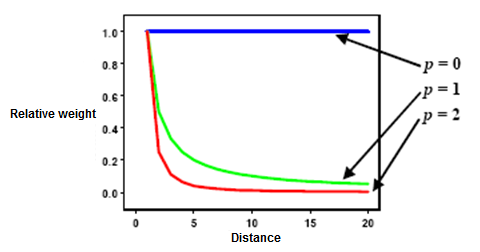
\includegraphics[width=.8\linewidth]{../writeup/images/idw_power.png}\\
		\textit{\footnotesize Source: ArcGIS Pro Help\\How inverse distance weighted interpolation works}
	\end{column}%
	\note{IDW is a method whereby the distance between a predicted point and a sample point is weighted.}
	\note{The underlying assumption is that there is a linear relationship between the location of the point of interest and the distance to the sample points.}
	\note{Sample points closest to the cell of interest are assumed to be more related to its value than those further away - flowingly, more weight is given to nearby points than to points in the distance}
	\note{Power values range from 0-3+ with a default settings generally being 2.}
	\note{A larger power value produces a more localized result - values further away from the cell have less impact on it's calculated value, values closer to the cell impact it values more.}
	\note{A smaller power value produces a more averaged result where sample points further away from the cell have a greater impact on the cell's calculated value.}
	\note{Larger power value = values further away have less impact}
	\note{Lower power value = values further away have a greater impact -> overall more average result}
\end{columns}
\end{frame}
\begin{frame}{Spline}
\begin{columns}[T] % align columns
	\begin{column}{.44\textwidth}
		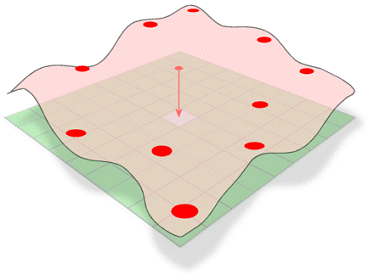
\includegraphics[width=.8\linewidth]{../writeup/images/spline.png}\\
		\textit{\footnotesize Spline \ldq{}rubber sheet\rdq{} fit to known data points \cite{albrecht_spline_2005}}
	\end{column}%
	\hfill%
	\begin{column}{.56\textwidth}
		\begin{itemize}
			\item Distortion through splines
			\item Minimizes overall surface curvature
			\item Creates a smooth continuous surface
			\item Bad for dense points with relatively high value differences
			\item Can estimate values outside of the measurement area
		\end{itemize}
	\end{column}%
\end{columns}
\end{frame}
\begin{frame}{Kriging}
\begin{columns}[T] % align columns
	\begin{column}{.52\textwidth}
		\begin{itemize}
			\item Geo-statistical approach
			\item Based on auto-correlation
			\item Produces a prediction surface
			\item Measure of certainty: error estimation and a confidence interval for every unknown point
		\end{itemize}
	\end{column}%
	\hfill%
	\begin{column}{.48\textwidth}
		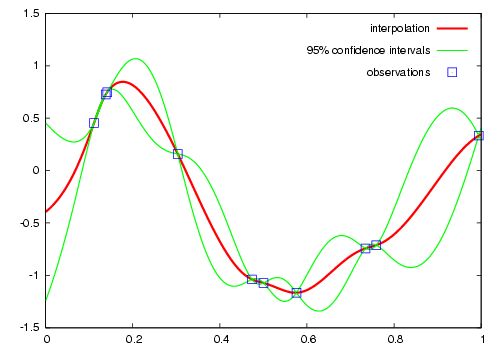
\includegraphics[width=\linewidth]{../writeup/images/kriging.png}\\
		\textit{\footnotesize Kriging in two dimensions \cite{gitta_raumliche_2016}}
	\end{column}%
\end{columns}
\end{frame}
\begin{frame}{Comparison Quiz}
\begin{minipage}{\textwidth}
	\centering
	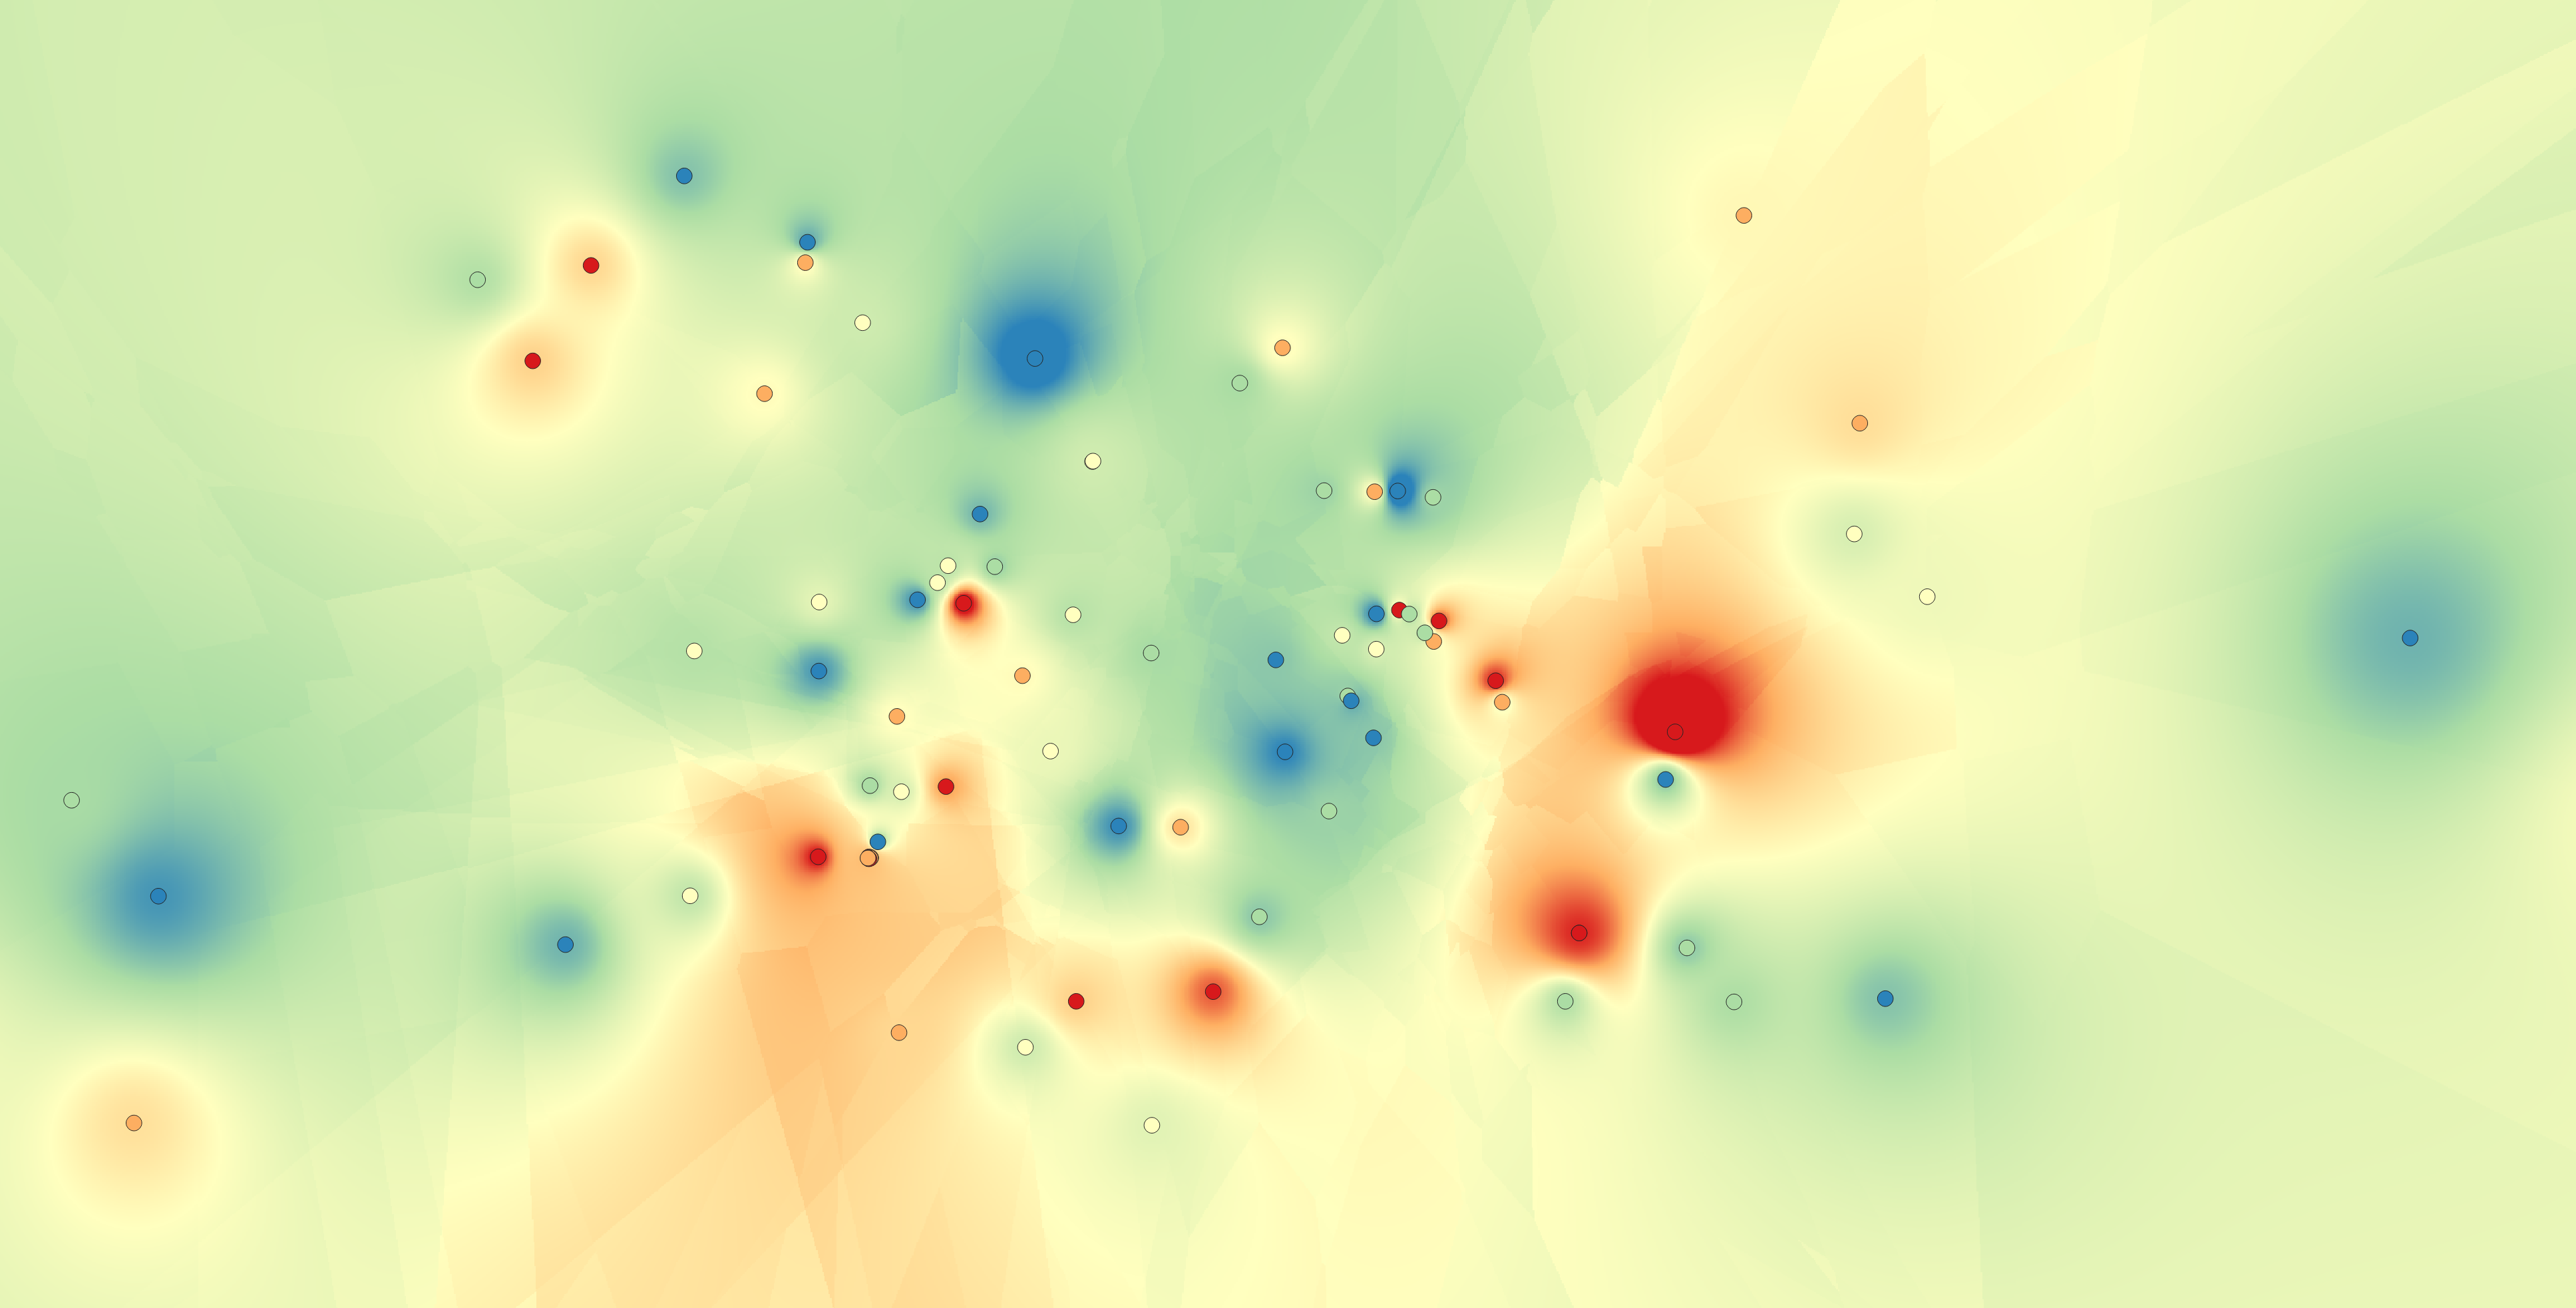
\includegraphics[width=5.5cm,keepaspectratio]{../writeup/images/interpolation_idw.png}\\
	\textit{\footnotesize
		\only<1>{Method 1}
		\only<2->{IDW}
	}
\end{minipage}
\vspace{0.5cm}\\
\begin{minipage}{0.5\textwidth}
	\centering
	% todo: NEAREST NEIGHBOR REDNERN
	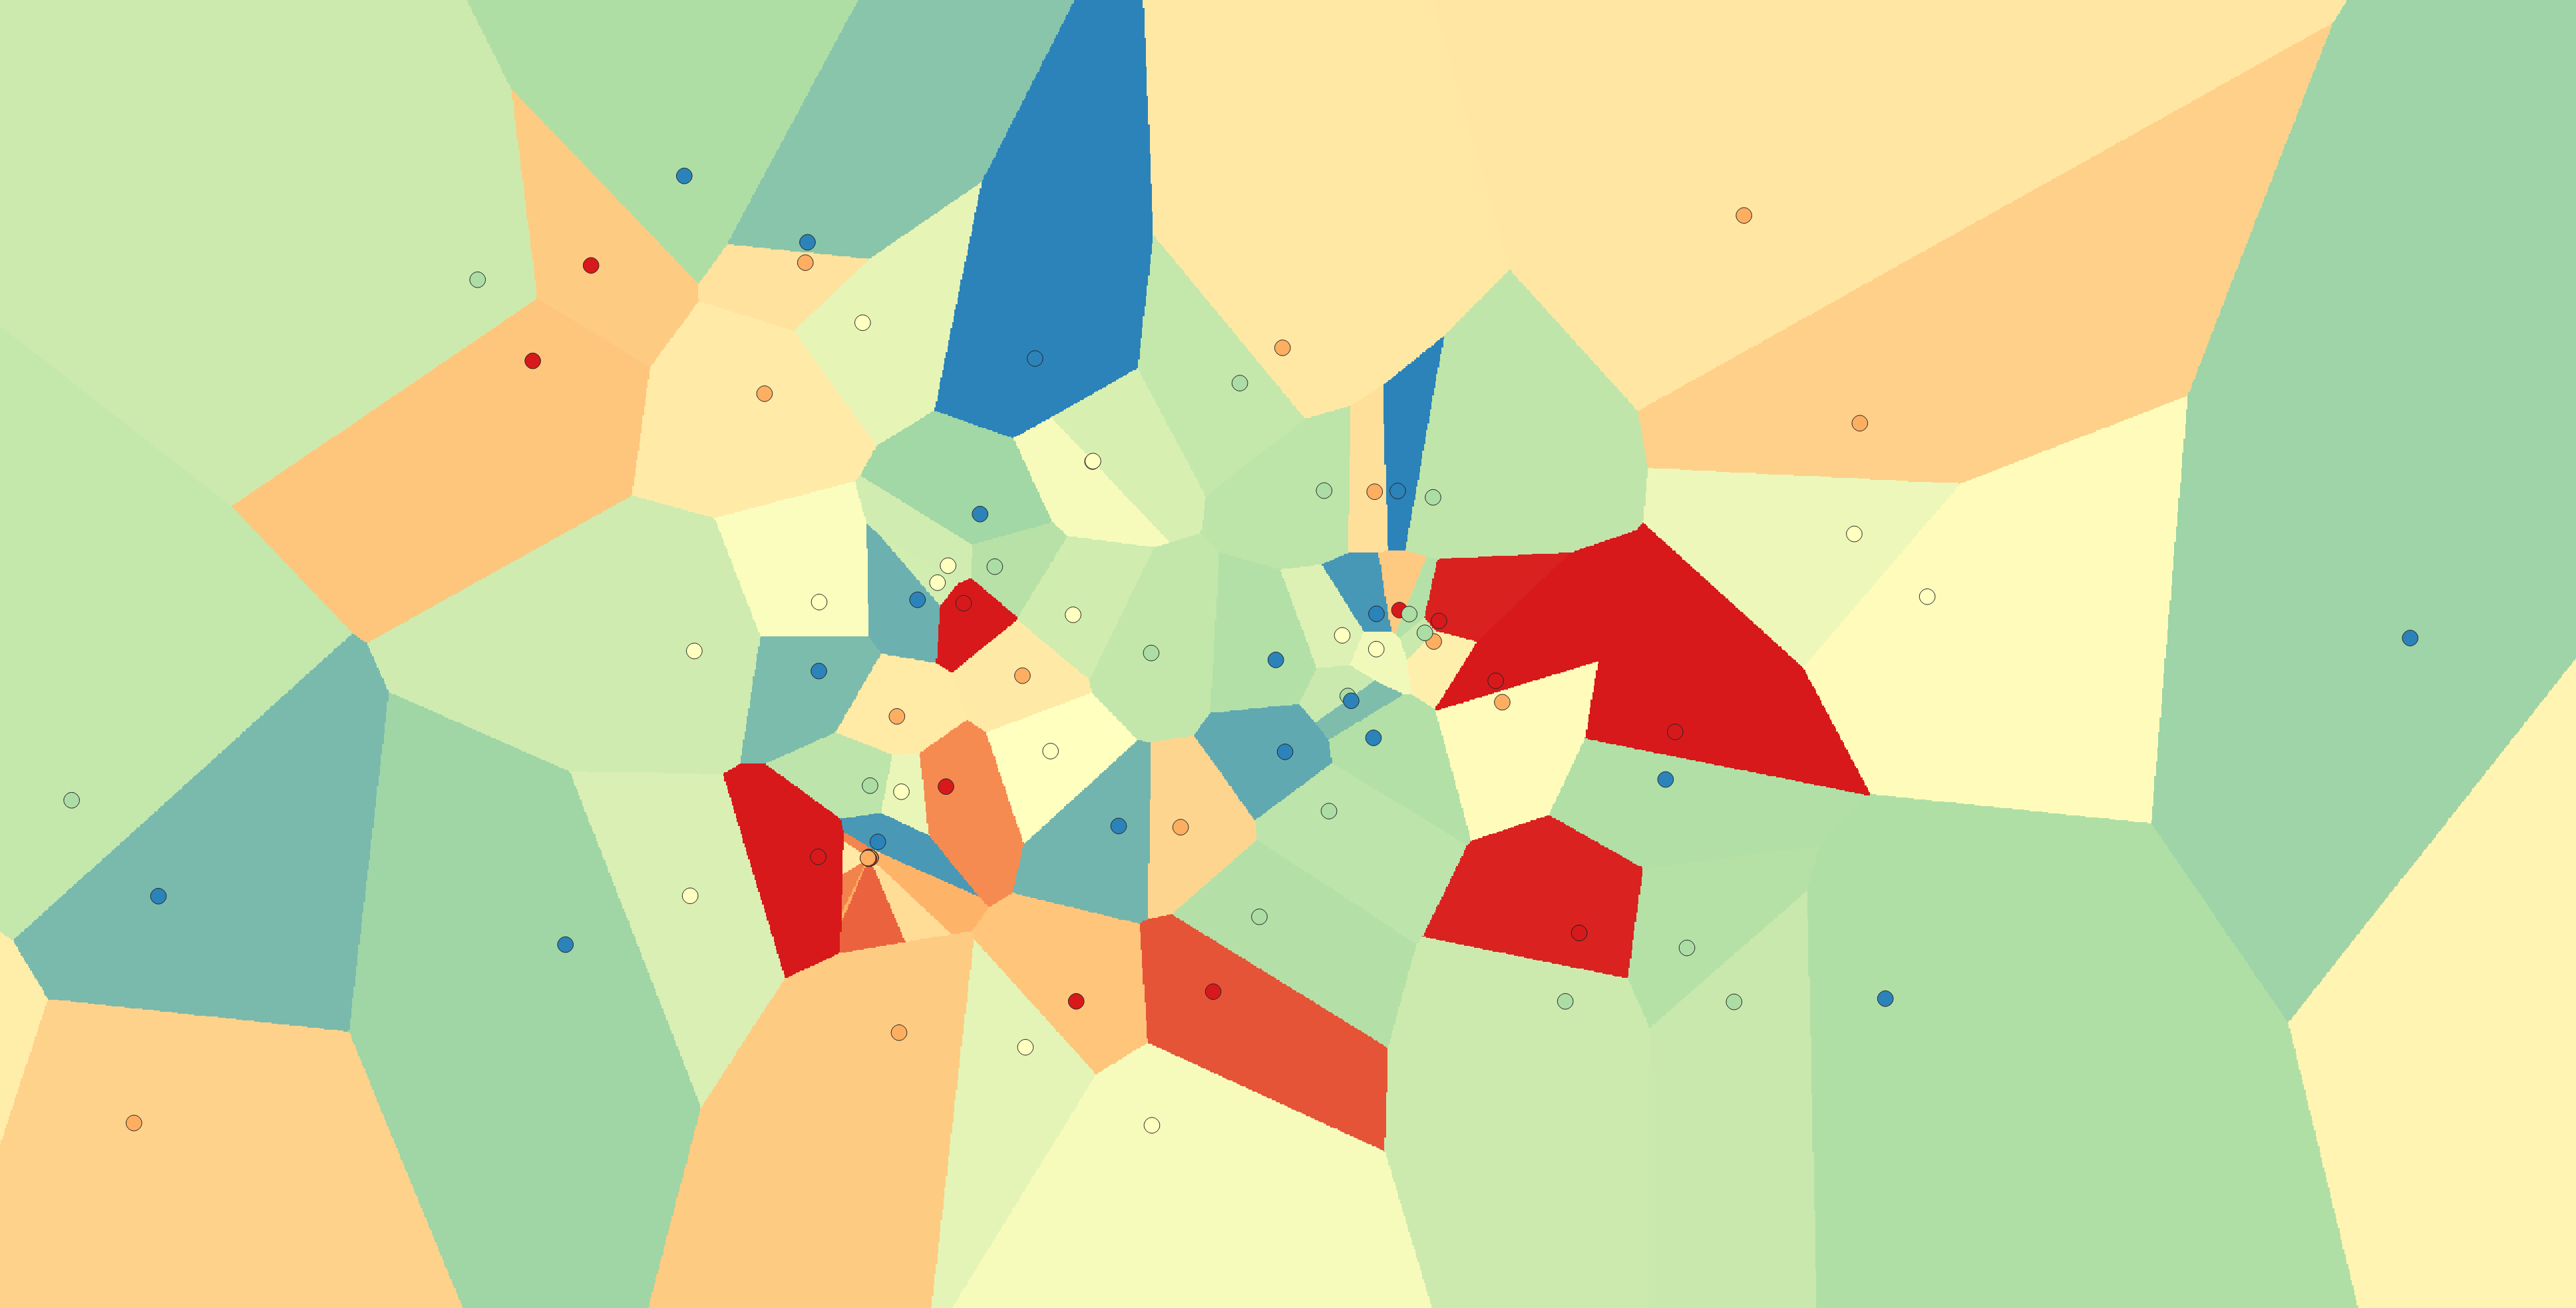
\includegraphics[width=5.5cm,keepaspectratio]{../writeup/images/interpolation_nearest.png}\\
	\textit{\footnotesize
		\only<1-2>{Method 2}
		\only<3->{Nearest Neighbor}
	}
\end{minipage}%
\begin{minipage}{0.5\textwidth}
	\centering
	\includegraphics[width=5.5cm,keepaspectratio]{../writeup/images/interpolation_TIN.png}\\
	\textit{\footnotesize
		\only<1-3>{Method 3}
		\only<4->{TIN}
	}
\end{minipage}
\end{frame}
\begin{frame}{Support in FOSSGIS tools}
\centering
\begin{tabular}{c|c|c|c|c}
	Interpolation method & QGIS & GRASS GIS & SAGA & GDAL\\
	\hline
	Nearest neighbor & \xmark &\cmark &\cmark & \cmark \\
	\hline
	TIN & \cmark &\cmark &\cmark & \cmark \\
	\hline
	IDW & \cmark &\cmark &\cmark & \cmark \\
	\hline
	Spline & \xmark &\cmark &\cmark & \xmark \\
	\hline
	Kriging & \xmark &\cmark &\cmark & \xmark \\
\end{tabular}
\end{frame}
	
	% !TeX root = ../presentation.tex

\section{Project}
\begin{frame}{Initial situation}
	\setbeamercovered{transparent}
	\begin{itemize}
		\item<1-> Use openSenseMap
		\item<2-> Get urban temperature sensors for Berlin
		\item<3-> Interpolate data using different methods 
		\item<4-> Create animation
		\item<5-> Compare results
	\end{itemize}
	\setbeamercovered{invisible}
\end{frame}
\begin{frame}{Problems: Getting the data}
\begin{columns}[c] % align columns
	\begin{column}{.52\textwidth}
		\begin{itemize}
			\item openSenseMap offers API access
			\item For bbox sensor data a phenomenon name must be given
			\item Phenomenon/Sensor name is a free-text field
			\item Different notations
			\item<2-> Most common one (Temperatur) was chosen
		\end{itemize}
	\end{column}%
	\hfill%
	\begin{column}{.48\textwidth}
		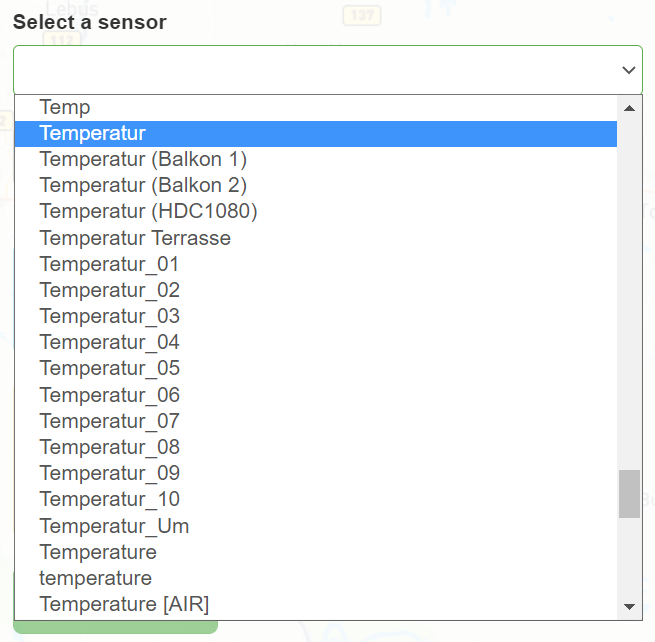
\includegraphics[width=\linewidth]{../writeup/images/phenomenon_name.png}
	\end{column}%
\end{columns}
\end{frame}
\begin{frame}{Problems: Aggregating data}
	\begin{itemize}
		\item Aggregated export does not cover full day
		\item Raw data may not include measurements throughout the day
		\item<2-> Manually aggregate raw data into 10 minute averages
		\item<2-> Filter out all stations that didn't provide measurements for every 10 minute interval
	\end{itemize}
\end{frame}
\begin{frame}{Problems: Data quality}
\begin{columns}[c] % align columns
	\begin{column}{.55\textwidth}
		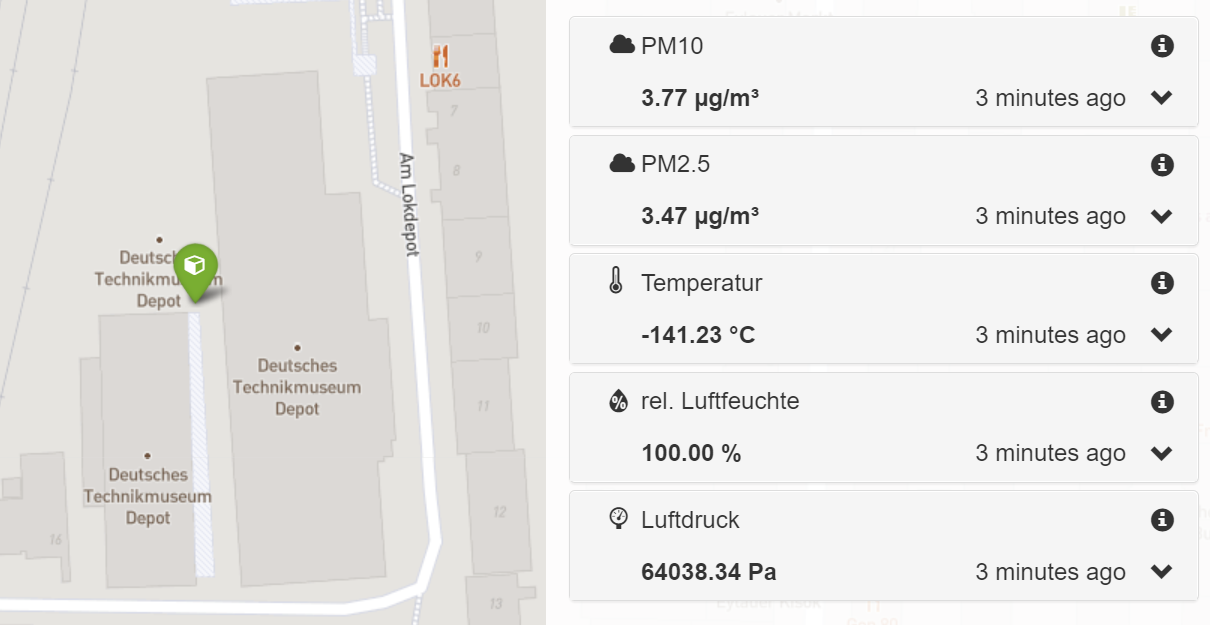
\includegraphics[width=\linewidth]{../writeup/images/outliers.png}
	\end{column}%
	\hfill%
	\begin{column}{.45\textwidth}
		\begin{itemize}
			\item Citizen-science project
			\item No validation of submitted data
			\item Do you spot any issues with the measurements?
			\item<2-> Filter all measurements that are more than double standard deviation from mean
		\end{itemize}
	\end{column}%
\end{columns}
\end{frame}
\begin{frame}{Final Workflow}
	\centering
	\scalebox{0.85}{
		\begin{tikzpicture}[node distance = 2cm, auto, every node/.style={color=text, fill=background, font=\sffamily}, align=center]
			% Place nodes
			\node [block] (in) {openSenseMap};
			\node [cloud, right=1.6cm of in, text width=7em] (avg) {Average\\into 10 minute intervals};
			\node [cloud, right=1.6cm of avg, text width=8em] (filter) {Filter\\by std deviation};
			\node [decision, below=1.6cm of filter] (interpolate) {Interpolate};
			\node [cloud, left=1.6cm of interpolate, text width=8em] (colorize) {Colorize\\1-band Tiff $\Rightarrow$ 4-band RGBA Tiff};
			\node [block, below=2.3cm of in] (out) {Generate frame};
			% Draw edges
			\draw [->] (in) -- (avg);
			\draw [->] (avg) -- (filter);
			\draw [->] (filter) -- (interpolate);
			\draw [->] (interpolate) -- (colorize);
			\draw [->] (colorize) -- (out);
		\end{tikzpicture}
	}
\end{frame}
	
	% !TeX root = ../presentation.tex

\section{Results}
\begin{frame}{Results}
	\begin{columns}[T] % align columns
		\begin{column}{.48\textwidth}
			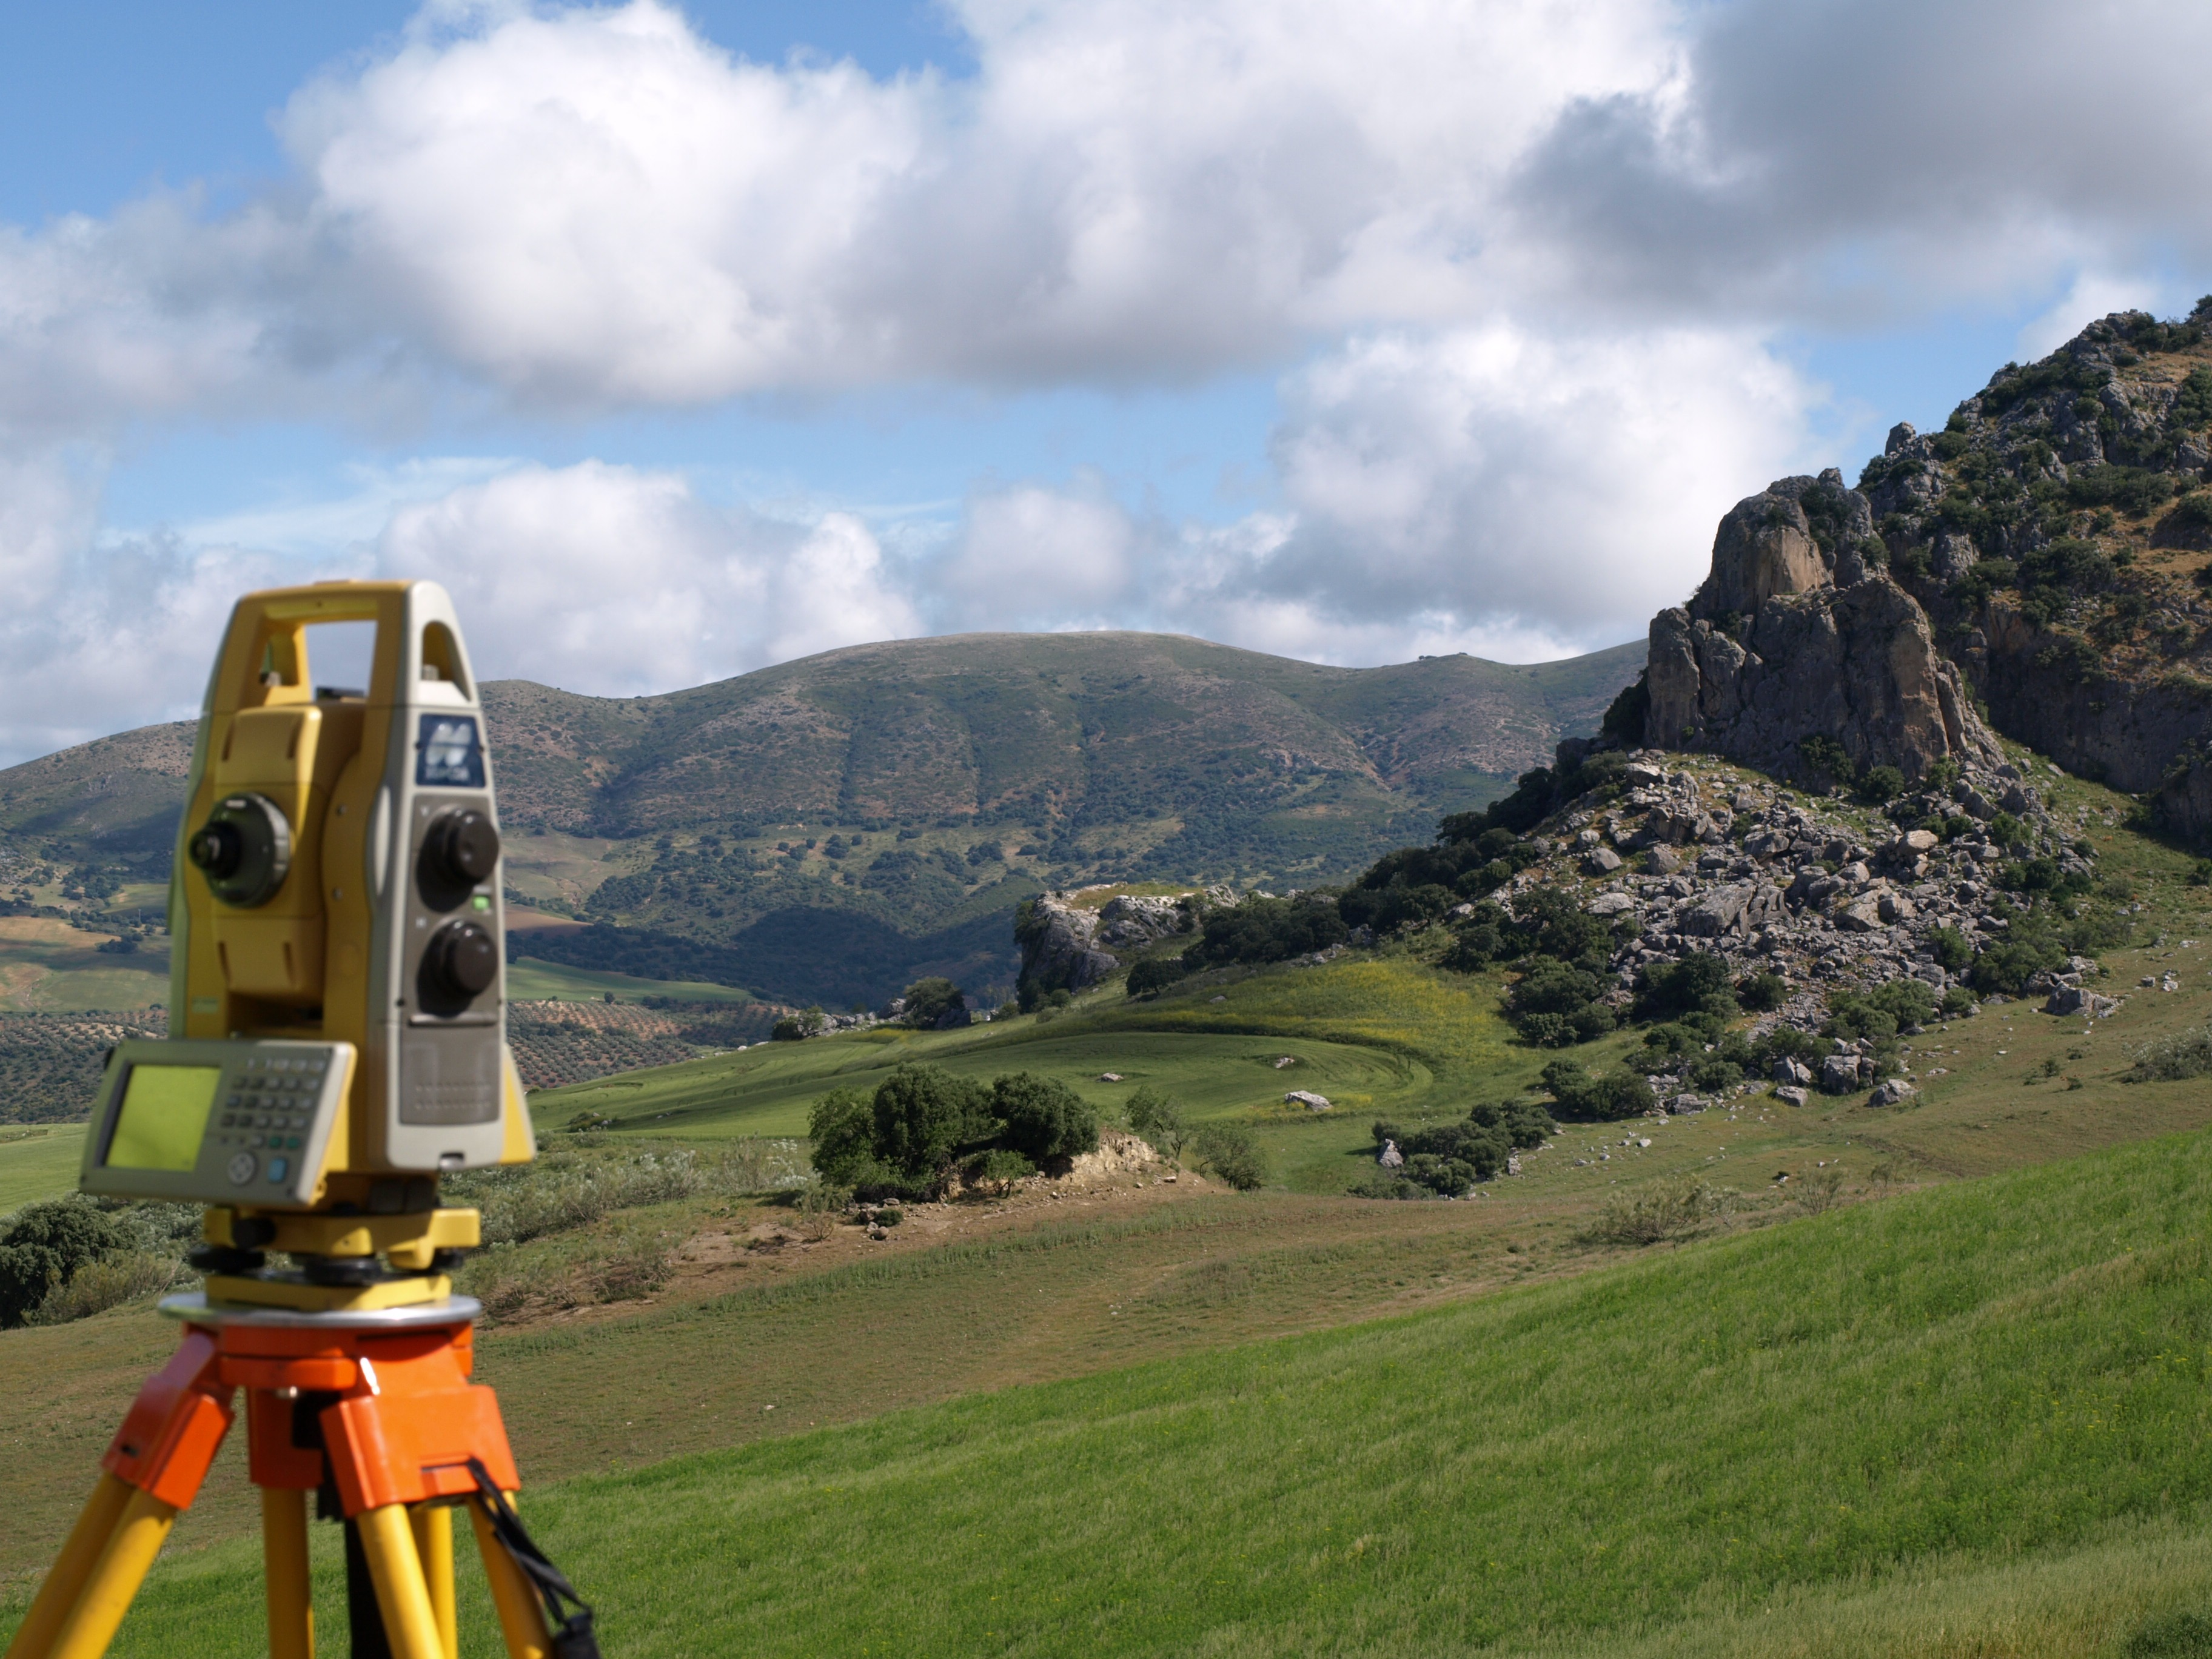
\includegraphics[width=\linewidth]{images/background}
		\end{column}%
		\hfill%
		\begin{column}{.56\textwidth}
			\begin{itemize}
				\item TODO
			\end{itemize}
		\end{column}%
	\end{columns}
	
\end{frame}
	
	% !TeX root = ../presentation.tex

\section{Outlook}
\begin{frame}{Outlook: Validation}
	\begin{itemize}
		\item Validate data internally
		\begin{itemize}
			\item Sample sets to check their accuracy
		\end{itemize}
		\item Validate data externally
		\begin{itemize}
			\item E.g. using DWD data
		\end{itemize}
	\end{itemize}
\end{frame}
\begin{frame}{Outlook: FOSSGIS comparison}
\begin{itemize}
	\item Check if implementation differs in different FOSSGIS tools
	\item Check for differences in default settings
	\begin{itemize}
		\item Which are better suited for our use case?
	\end{itemize}
\end{itemize}
\end{frame}
	
%	{
%		\metroset{sectionpage=none,numbering=none}
%		\section{Demo}
%		\begin{frame}[standout]
%			\begin{env}
%				\usebeamercolor[fg]{normal text}
%				\LARGE
%				DEMO
%			\end{env}
%		\end{frame}
%	}

	% !TeX root = ../presentation.tex

\appendix

\begin{frame}{Appendix}
	TODO
\end{frame}
	
\end{document}
